\documentclass[]{article}

% Imported Packages
%------------------------------------------------------------------------------
\usepackage{amssymb}
\usepackage{amstext}
\usepackage{amsthm}
\usepackage{amsmath}
\usepackage{enumerate}
\usepackage{fancyhdr}
\usepackage[margin=1in]{geometry}
\usepackage{graphicx}
\usepackage{extarrows}
\usepackage{setspace}
\usepackage{float}
%------------------------------------------------------------------------------

% Header and Footer
%------------------------------------------------------------------------------
\pagestyle{plain}  
\renewcommand\headrulewidth{0.4pt}                                      
\renewcommand\footrulewidth{0.4pt}                                    
%------------------------------------------------------------------------------

% Title Details
%------------------------------------------------------------------------------
\title{Deliverable \#3: What’s That Dish Software}
\author{SE 3A04: Software Design II -- Large System Design}
\date{}                               
%------------------------------------------------------------------------------

% Document
%------------------------------------------------------------------------------
\begin{document}

\maketitle	
\noindent{\bf Tutorial Number:} T03\\
{\bf Group Number:} G03 \\
{\bf Group Members:} 
\begin{itemize}
	\item Imran Chowdhury
	\item Michael Roberts
	\item Sathurshan Arulmohan
	\item Tanisha Tasnin
	\item Zifan Si
\end{itemize}

\section{Introduction}
\label{sec:introduction}
% Begin Section

This section should provide an brief overview of the entire document.

\subsection{Purpose}
\label{sub:purpose}
% Begin SubSection

This document provides further detail on the architecure and design of \textit{What's that Dish}, including state diagrams for controller classes,
sequence diagrams and the detailed class diagram. It compliments Deliverables 1 and 2, which all readers are advised to familarize themselves with
to further their understanding of this document.

This document is intended for internal technical stakeholders, including, but not limited to, developers, domain experts,
and engineering managers. It may have some use to non-technical stakeholders, including non-engineering project managers,
senior executives, investors, restarants, and future end users.
% End SubSection

\subsection{System Description}
\label{sub:system_description}
% Begin SubSection
A sucinct description is contained in Deliverable 2. This document is meant to supplement Deliverable 2 through providing 
state charts for controller classes, sequence diagrams and a detailed class diagram.

% End SubSection

\subsection{Overview}
\label{sub:overview}
% Begin SubSection
The document will present the state diagram of each controller from the class analysis diagram in section 2.
Section 3 will provide sequence diagrams for each use case of \textit{What's That Dish}.
Finally section 4 shows the detailed class diagram of the application.

% End SubSection

% End Section

\section{State Charts for Controller Classes}
\label{sec:state_charts_for_controller_classes}
% Begin Section
\begin{figure}[H]
	\centering
   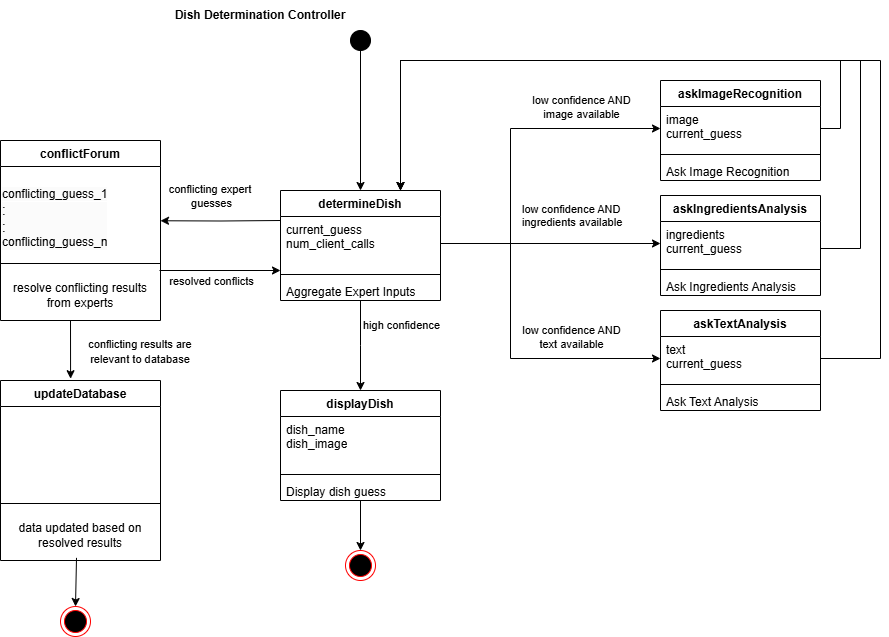
\includegraphics[width=\textwidth]{image/D3_state_diagrams/dish_determination.png}
\end{figure}

\begin{figure}[H]
	\centering
   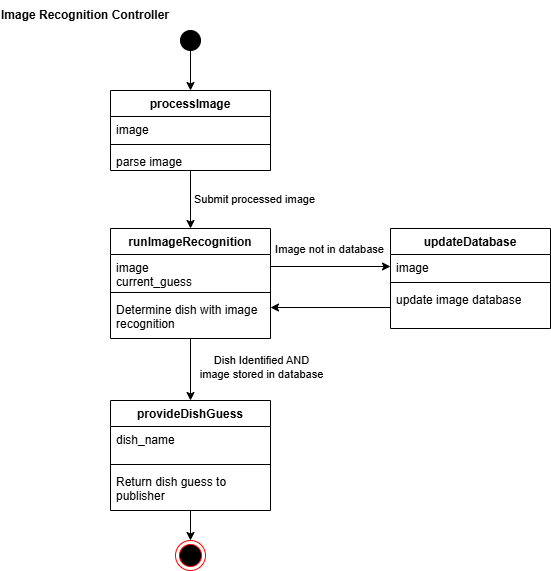
\includegraphics[width=\textwidth]{image/D3_state_diagrams/image_recognition.png}
\end{figure}

\begin{figure}[H]
	\centering
   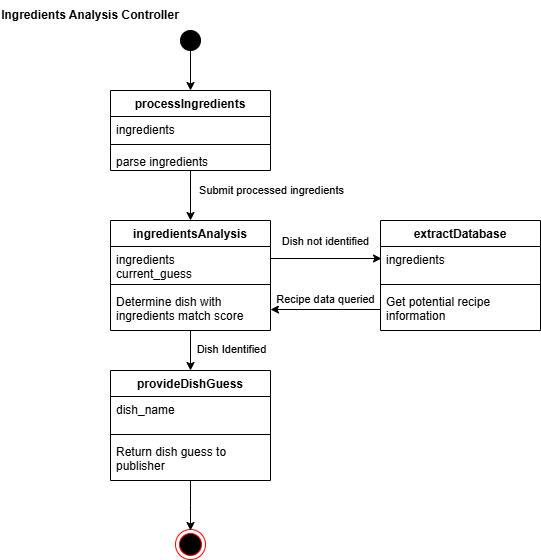
\includegraphics[width=\textwidth]{image/D3_state_diagrams/ingredients_analysis.png}
\end{figure}


\begin{figure}[H]
	\centering
   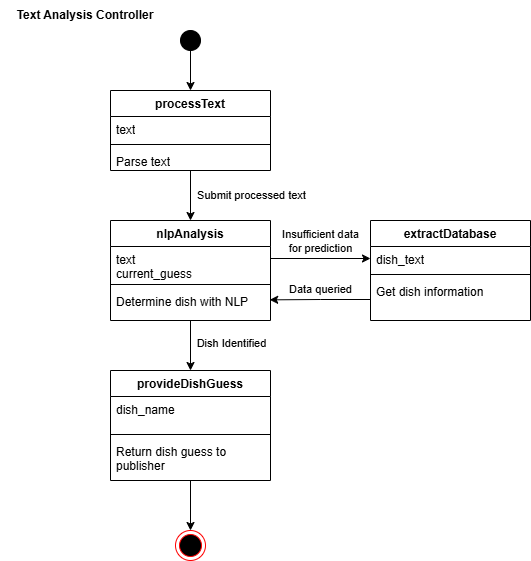
\includegraphics[width=\textwidth]{image/D3_state_diagrams/text_analysis.png}
\end{figure}

\begin{figure}[H]
	\centering
   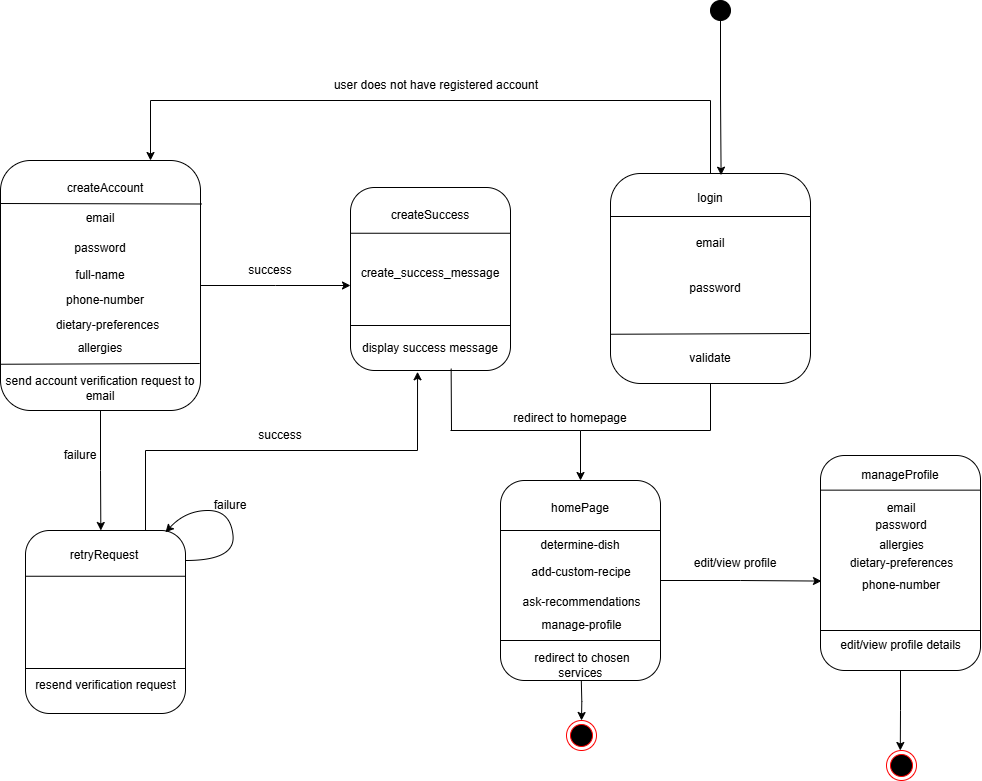
\includegraphics[width=\textwidth]{image/D3_state_diagrams/account_management.png}
\end{figure}

\begin{figure}[H]
	\centering
   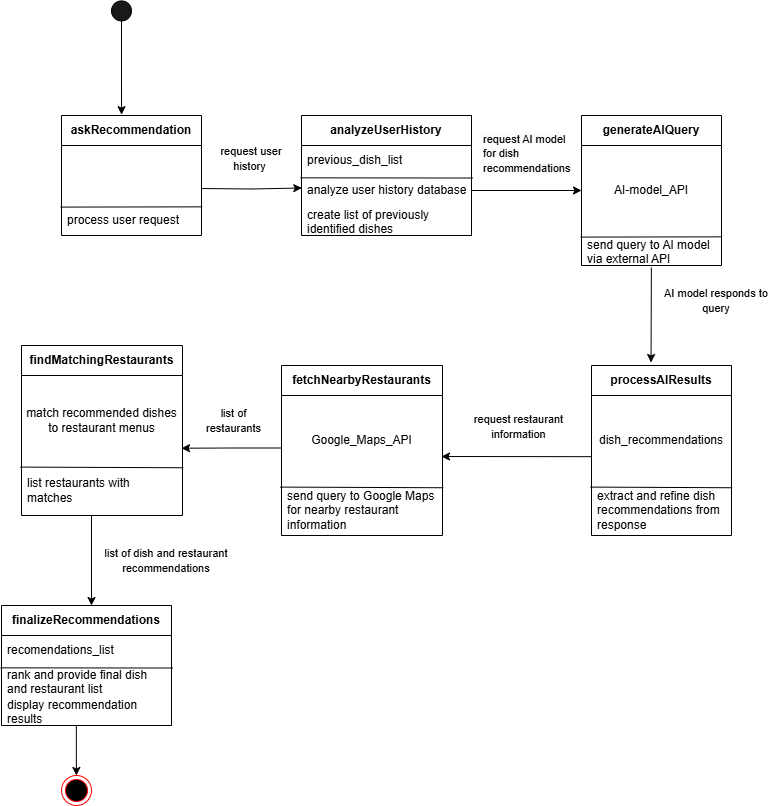
\includegraphics[width=\textwidth]{image/D3_state_diagrams/recommendation_system.png}
\end{figure}

\begin{figure}[H]
	\centering
   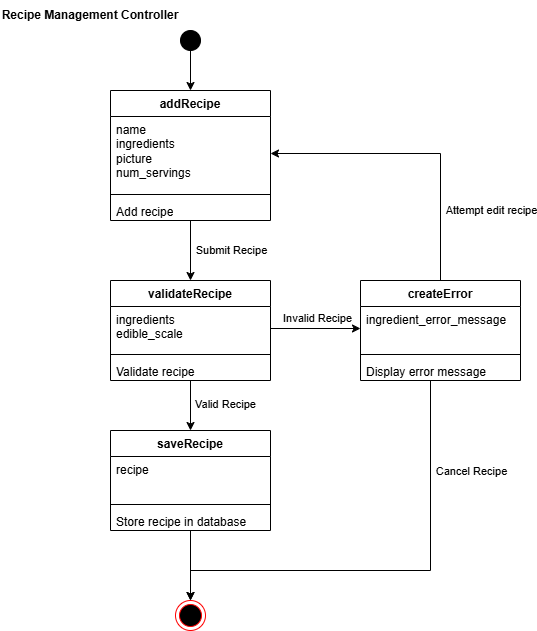
\includegraphics[width=\textwidth]{image/D3_state_diagrams/recipe_management.png}
\end{figure}

% End Section

\section{Sequence Diagrams}
\label{sec:sequence_diagrams}
% Begin Section
This section should provide a sequence diagram for each use case of your application.
% End Section

\section{Detailed Class Diagram}
\label{sec:detailed_class_diagram}
% Begin Section
\begin{figure}[H]
	\centering
   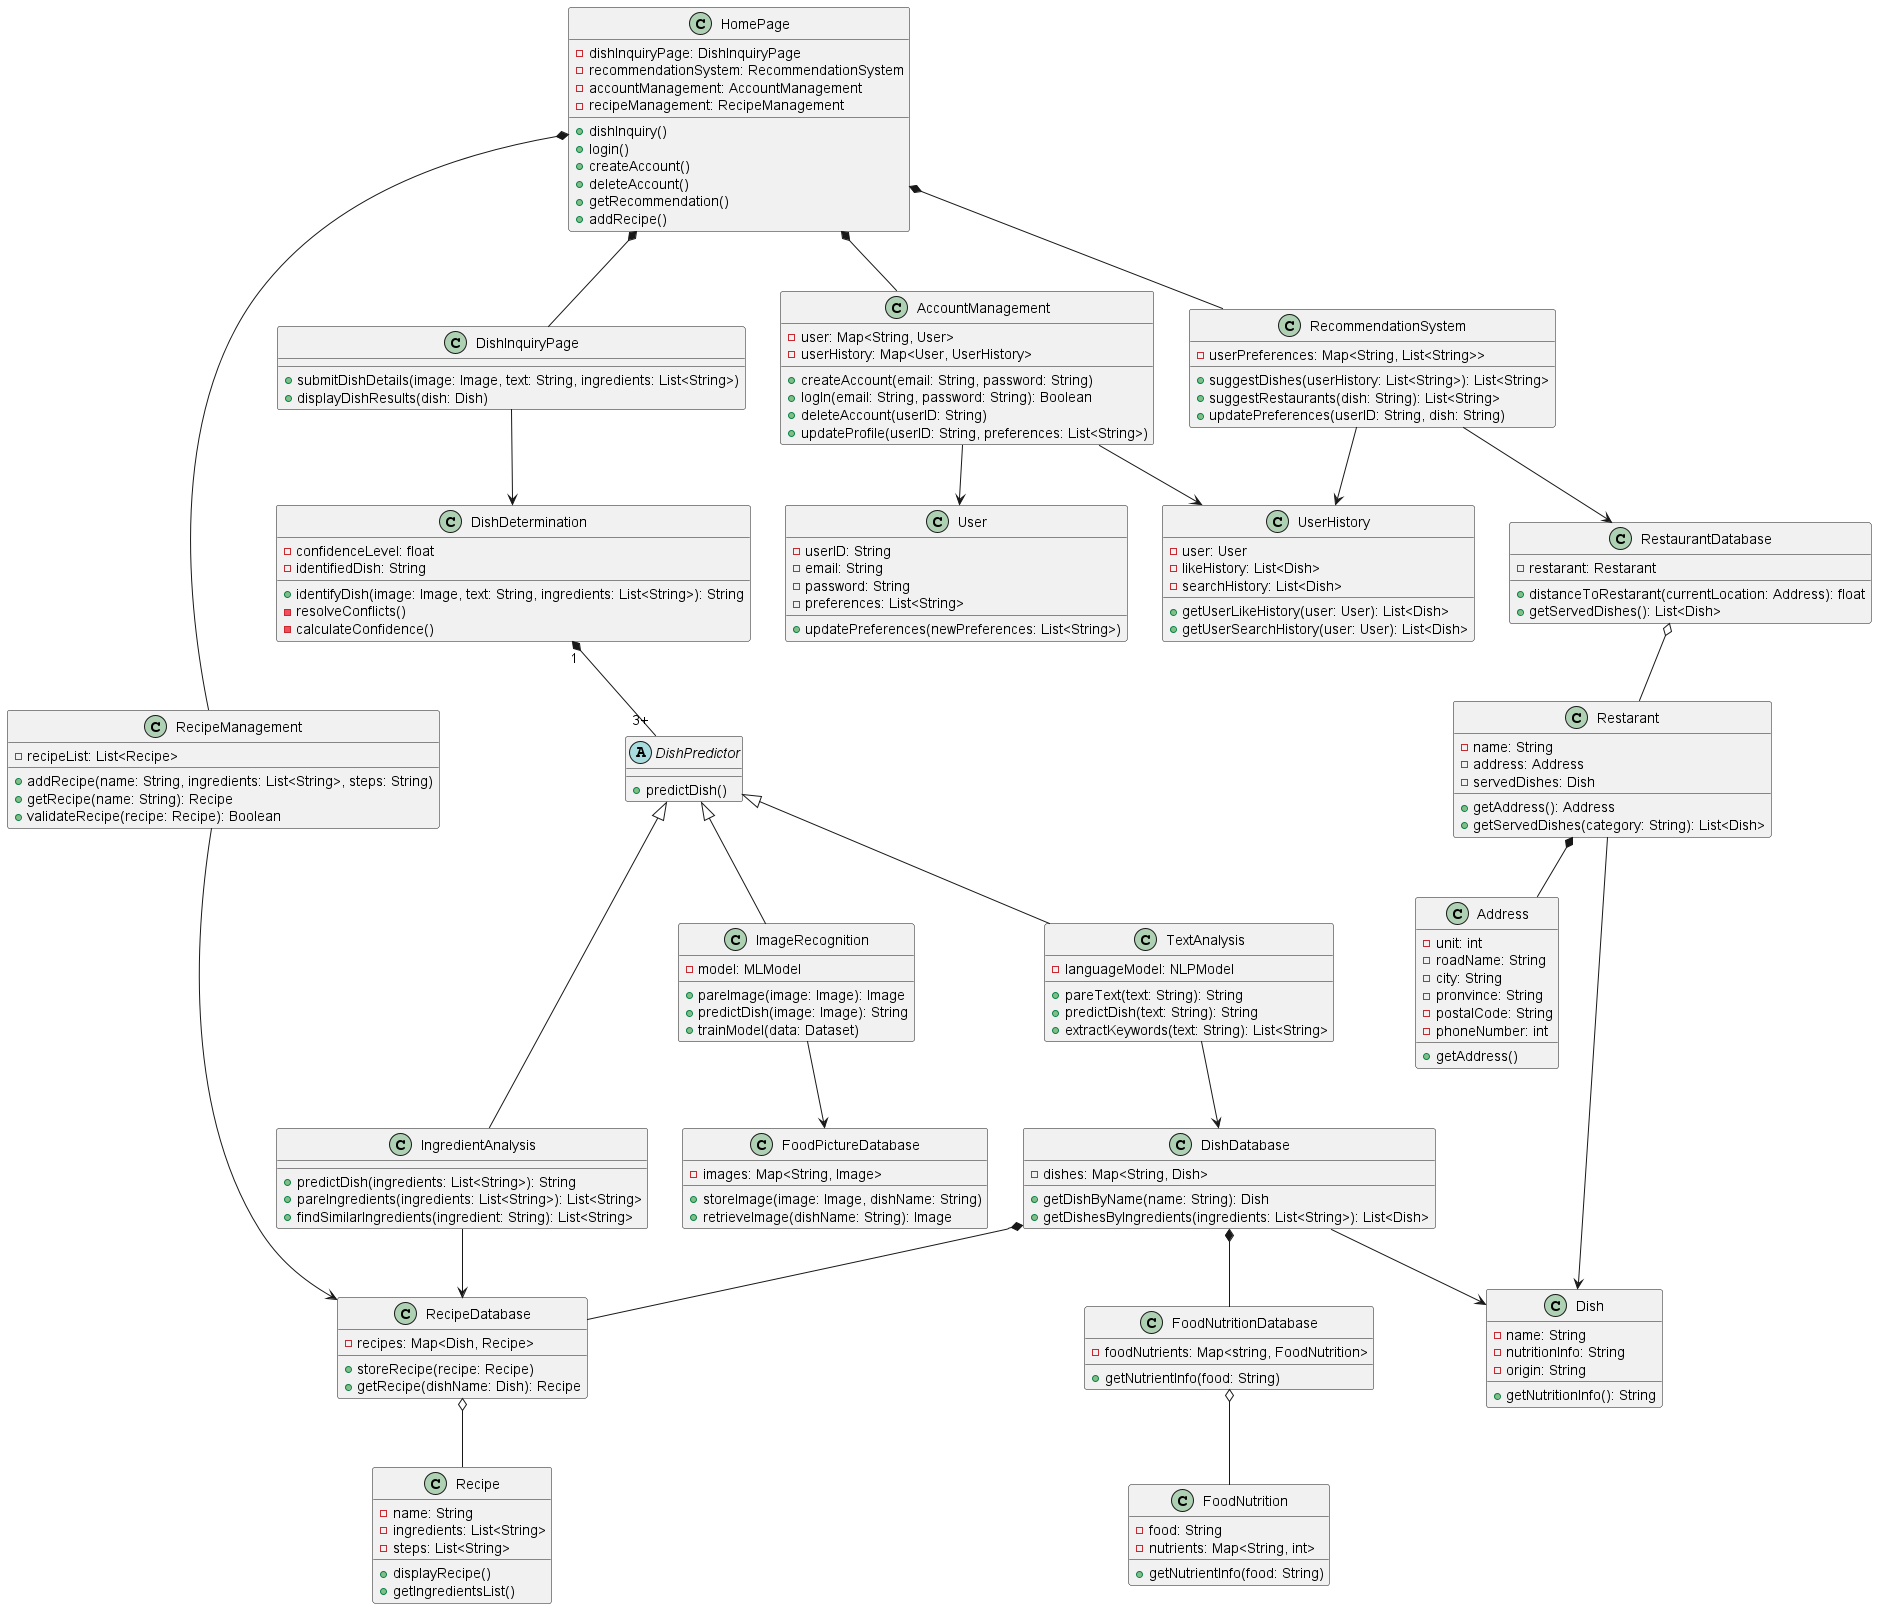
\includegraphics[width=\textwidth]{image/detailedClassDiagram.png}
\end{figure}

% End Section

\appendix
\section{Division of Labour}
\label{sec:division_of_labour}
% Begin Section
\textbf{Imran Chowdhury:}
\begin{enumerate}
	\item TODO
\end{enumerate}

\textbf{Signature:} Imran Chowdhury \\

\textbf{Michael Roberts:}
\begin{enumerate}
	\item Drafted Sections 1.1 and 1.2.
	\item Drafted and revised class diagram with Zifan.
\end{enumerate}

\begin{figure}[H]
 	\centering
    
\includegraphics[width=\textwidth]{image/A_Michael_Roberts_Signature.png}
\end{figure}

\textbf{Sathurshan Arulmohan:}
\begin{enumerate}
	\item Developed state diagrams for recipe management, image recognition, text analysis, and ingredients analysis controllers.
	\item Worked with Tanisha on state diagram for dish determination.
	\item Reviewed and provided feedback for state diagrams for recommendation system and account managerment controller.
	\item Edited the detailed class diagram.
	\item Wrote section 1.3.
\end{enumerate}

\textbf{Signature:} SATHURSHAN ARULMOHAN \\

\textbf{Tanisha Tasnin:}
\begin{enumerate}
	\item TODO
\end{enumerate}

\textbf{Signature:} TANISHA TASNIN \\

\textbf{Zifan Si:}
\begin{enumerate}
	\item Worked on part 4 class diagram.
	\item add fix to D2 3.2 based on feedback.
\end{enumerate}

\textbf{Signature:} ZIFAN SI  \\
% End Section

\newpage
\section*{IMPORTANT NOTES}
\begin{itemize}
	\item You do \underline{NOT} need to provide a text explanation of each diagram; the diagram should speak for itself
	\item Please document any non-standard notations that you may have used
	\begin{itemize}
		\item \emph{Rule of Thumb}: if you feel there is any doubt surrounding the meaning of your notations, document them
	\end{itemize}
	\item Some diagrams may be difficult to fit into one page
	\begin{itemize}
		\item It is OK if the text is small but please ensure that it is readable when printed
		\item If you need to break a diagram onto multiple pages, please adopt a system of doing so and throughly explain how it can be reconnected from one page to the next; if you are unsure about this, please ask me
	\end{itemize}
	\item Please submit the latest version of Deliverable 1 and Deliverable 2 with Deliverable 3
	\begin{itemize}
		\item They do not have to be a freshly printed versions; the latest marked versions are OK
	\end{itemize}
	\item If you do \underline{NOT} have a Division of Labour sheet, your deliverable will \underline{NOT} be marked
\end{itemize}


\end{document}
%------------------------------------------------------------------------------